\chapter{Основы релятивистской теории}

Традиционная квантовая механика, базирующаяся на уравнении Шрёдингера и теории спина Паули, вызывает известное чувство неудовлетворенности теми обстоятельствами, что:

\begin{sloppypar}
\begin{enumerate}
\item{Теория оказывается не инвариантной относительно преобразований Лоренца\footnotemark (или не является лоренц-ковариантной), как того требует принцип относительности. Причина в том, что основное уравнение --- уравнение Шрёдингера --- \underline{нерелятивистское}}
\item{Спин в теории Паули вводится <<руками>>, а не следует из основ теории.}
\end{enumerate}
\end{sloppypar}
%people
\footnotetext{Хендрик Антон Лоренц (Hendrik Antoon Lorentz, 1853-1928)}

Поэтому необходимо обобщение уравнения Шрёдингера на релятивистский случай и формулировка всей теории в лоренц-ковариантной форме. Именно на этом пути удается достичь существенного прогресса в вопросе происхождения спина элементарных частиц (в частности, электрона), обосновывая {\em гипотезу Уленбека-Гаудсмита}\footnotemark (1925 г.)
%people
\footnotetext{Джордж Юджин Уленбек (George Eugene Uhlenbeck, 1900-1988); Сэмюэл Абрахам Гаудсмит (Samuel Abraham Goudsmit, 1902-1978)}

Предметом нашего дальнейшего рассмотрения будет {\em релятивистская квантовая механика}, в которой будет допущен ряд идеализаций:
\begin{enumerate}
\item{Частицы считаются {\em точечными} (без внутренней структуры). Согласно экспериментальным данным по рассеянию, установлена точечность электрона до $10^{-18}$ см. Однако общеизвестно, что, например, нуклоны имеют кварковую структуру.}

\item{{\em Изолированность частиц.} Это понятие становится все более относительным, т.~к. фундаментален факт взаимопревращений частиц при реакциях.}
\item{{\em Сохранение числа частиц}. В физике высоких энергий (${E > mc^2}$) это положение теряет смысл. Здесь все более значительной становится роль процессов с изменением числа частиц и превращения частиц (рождение и аннигиляция частиц). Полное релятивистское квантовое описание таких процессов приводит к понятию квантованных полей, а соответствующая теория называется {\em квантовой теорией поля.}}
\end{enumerate}

Наше рассмотрение будет касаться предварительного этапа: мы будем считать, что число частиц \underline{постоянно} (т.~е. пренебрежем процессами с изменением числа частиц), а уравнение --- \underline{релятивистское}, т.~е. пригодное для описания частиц высоких энергий (${E \ge m_e c^2 = 0.5}$ МэВ). На этом пути мы используем одночастичный подход, т.~е. рассматривается релятивистская квантовая механика одной изолированной частицы.

\section{Уравнение Дирака (1928 г.) свободной релятивистской частицы}

В 25 лет английский физик-теоретик построил фундамент современной квантовой физики, предложив волновое релятивистское уравнение, описывающее движение не только \underline{электронов}, но и их античастиц --- \underline{позитронов}.

Перейдем теперь к построению релятивистского волнового уравнения, которое могло бы описывать частицы со спином $s = 1/2$, например, электроны. В нерелятивистской теории электрон описывается {\em паулиевским} (или двухкомпонентным) спинором, т.~е. волновой функцией $\psi(\vr, t) = \brc{\begin{matrix} \psi_1 \\ \psi_2\end{matrix}}$, компоненты которой при трехмерных вращениях преобразуются как компоненты углового момента, равного $1/2$. Поэтому, если мы хотим построить релятивистское обобщение спинора Паули, то необходимо заложить в теорию возможность описания частицы многокомпонентной волновой функцией, компоненты которой преобразуются друг через друга вполне определенным образом при преобразованиях Лоренца.

Как и в нерелятивистской теории, волновую функцию $\Psi$ в данный момент времени $t$ можно рассматривать как функцию пространственных координат $\vr$ и внутренних, или спиновых, переменных $s$. Такая функция задает некоторый вектор состояния частицы $\ket{\Psi(t)}$ в гильбертовом пространстве состояний $\mathcal{H} = \mathcal{H}^{\text{орб}} \otimes \mathcal{H}^{\text{спин}}$ (прямое произведение пространства орбитального движения на пространство спиновой переменной):
$$
\Psi(\vr, t, s) = \Psi_s(\vr, t) = \bk{\vr, s}{\Psi(t)}
$$
(проекция вектора состояний $\ket{\Psi(t)}$ в некоторой точке $\ket{\vr, s}$ спин-орбитального пространства $H$ --- см. \S 3 главы \rom{6})

\begin{defn}
Прямым (тензорным) произведением пространств $\epsilon_a$ и $\epsilon_b$ называется $n_a~n_b$-мерное пространство $\epsilon_a \otimes \epsilon_b$, базисными векторами которого являются векторы $\ket{a \mu b \nu} \equiv \ket{a \mu}\ket{b \nu}$, где  
$\mu = 1, 2, \dots, n_a$; $\nu = 1, 2, \dots, n_b$.
\end{defn}

По аналогии с теорией Паули функцию $\Psi(\vr, t, s)$ представим в виде столбца из $N$ компонент $\Psi_s(\vr, t)$ ($s$ --- номер компоненты): $\mathsf{\Psi}(\vr, t) = 
\brc{\begin{matrix}
\Psi_1 \\
... \\
\Psi_N
\end{matrix} }
$.

Далее предположим, что искомое уравнение можно записать в гамильтоновой форме:
\begin{equation}
\label{eq:14_1_1}
i\hbar \pd{}{t} \mathsf{\Psi}(\vr, t) = \op{H}_D \mathsf{\Psi}(\vr, t),
\end{equation}
где $\op{H}_D$ --- гамильтониан Дирака, соответствующий линеаризованной форме выражения для релятивистской энергии частицы:
\begin{equation}
\label{eq:14_1_2}
E = \sqrt{c^2 \vp^2 + m^2 c^4}
\end{equation}
 
Линеаризация радикала необходима потому, что левая часть \eqref{eq:14_1_1} линейна по $\pd{}{t}$ (\underline{уравнение первого порядка по времени}), а т.~к. искомое уравнение должно быть релятивистски инвариантным к преобразованиям Лоренца, то оно должно отражать равноправие пространственных и временных переменных, т.~е. должно быть \underline{уравнением первого порядка и по пространственным переменным}. Иными словами, гамильтониан $\op{H}_D$ свободной релятивистской частицы должен быть линейной функцией компонент оператора импульса 
$$
\op{p}_i = - i\hbar \pd{}{x_i}
$$

\subsection{<<Линеаризация корня>>}

Следуя Дираку, попытаемся, введя 4 матричных коэффициента $\op{\alpha}_i$ ($i = 1, 2, 3$) и $\op{\beta}$, представить \eqref{eq:14_1_2} в виде:
\begin{equation}
\label{eq:14_1_3}
E \op{1} = \sqrt{c^2 \vp^2 + m^2 c^4} \op{1} = c \sum_{i=1}^3 (\op{\alpha}_i p_i) + \op{\beta} mc^2 \equiv c(\aD \cdot \vp) + \op{\beta} mc^2,
\end{equation}
где $\op{1}$ --- единичная матрица размера $N \times N$. Определим, каким условиям должны удовлетворять введенные объекты $\op{\alpha}_i$ и $\op{\beta}$. Для этого возведем последнее выражение в квадрат:
\begin{gather}
E^2 \op{1} = (c^2 \vp^2 + m^2 c^4)\op{1} = \brcr{c \sum_{i=1}^3 (\op{\alpha}_i p_i) + \op{\beta} mc^2} \times \brcr{c \sum_{j=1}^3 (\op{\alpha}_j p_j) + \op{\beta} mc^2} = \nonumber \\
\label{eq:14_1_4}
= {c^2 \sum_{i=1}^3 \sum_{j = 1}^3 (\op{\alpha}_i, p_i)(\op{\alpha}_j, p_j)} + mc^3 \sum_{i=1}^3 (\op{\alpha}_i \op{\beta} + \op{\beta} \op{\alpha}_i) p_i + \op{\beta}^2 m^2 c^4
\end{gather}

Первое слагаемое в правой части \eqref{eq:14_1_4} удобно переписать в симметризованном виде:
$$
c^2 \sum_{i=1}^3 \sum_{j = 1}^3 \frac{ \op{\alpha}_i \op{\alpha}_j + \op{\alpha}_j \op{\alpha}_i }{2} p_i p_j
$$

\begin{excr}
Доказать это утверждение.
\end{excr}

Равенство \eqref{eq:14_1_4} будет выполняться, если объекты $\op{\alpha}_i$ и $\op{\beta}$ подчиняются следующей алгебре:
\begin{eqnarray}
\label{eq:14_1_5}
  \brcr{\op{\alpha}_i, \op{\alpha}_j } \equiv \op{\alpha}_i \op{\alpha}_j  + \op{\alpha}_j \op{\alpha}_i = 2 \delta_{ij} \op{1}; \nonumber \\
  \brcr{\op{\alpha}_i, \op{\beta} } \equiv \op{\alpha}_i \op{\beta} + \op{\beta} \op{\alpha}_i = 0;~~~\op{\beta}^2 = \op{1} = \op{\alpha}_i^2.
\end{eqnarray}

То есть все эти объекты должны \underline{антикоммутировать}, а квадрат каждого из них должен быть равен $\op{1}$. Заметим, что $\op{\alpha}_i$ и $\op{\beta}$ не могут быть действительными или комплексными числами, т.~к. числа коммутируют между собой, но не антикоммутируют. Если $\op{\alpha}_i$ и $\op{\beta}$ считать \underline{матрицами}, то выше были получены матричные уравнения \eqref{eq:14_1_5}, и искомое релятивистское волновое уравнение должно быть \underline{матричным уравнением}. Причем число компонент волновой функции $\mathsf{\Psi}(\vr, t)$ должно совпадать с размерностью матриц $\op{\alpha}_i$ и $\op{\beta}$. 

Произведя в \eqref{eq:14_1_3} замену классических величин на операторы:
${E \to i\hbar \pd{}{t};~~~\vp \to \op{\vp} = -i \hbar \vec{\nabla},}$
получим уравнение Дирака в виде \eqref{eq:14_1_1}, где
\begin{equation}
\label{eq:14_1_6}
\boxed{\op{H}_D = c(\aD, \op{\vec{p}}) + \op{\beta} mc^2}
\end{equation}
--- гамильтониан Дирака. Из вида гамильтониана и его эрмитовости следует:
$$
\boxed{\op{\alpha}_i^\dag = \op{\alpha}_i,~~\op{\beta}^\dag = \op{\beta}}
$$

\begin{excr}
Доказать это утверждение.
\end{excr}

Из \eqref{eq:14_1_6} ясно, что операторы $\op{\alpha}_i$ и $\op{\beta}$ действуют только в пространстве спиновых переменных $\mathcal{H}^{\text{спин}}$. Что собой представляет это пространство?

\subsection{Матрицы Дирака и их свойства}

Напомним, что любая эрмитова матрица всегда может быть диагонализирована с помощью подходящей унитарной матрицы $\op{U}$ ($\op{U} \op{U}^\dag = \op{U}^\dag \op{U} = \op{1}$, см. \S 2 главы \rom{6}). То есть, например, для матрицы $\op{\beta}$ всегда может быть подобрана такая унитарная матрица $\op{U}$, что $\op{\beta}' = \op{U} \op{\beta} \op{U}^\dag$ станет диагональной матрицей.

Из условий \eqref{eq:14_1_5} $\op{\alpha}_i^2 = \op{\beta}^2 = \op{1}$ следует, что собственными значениями матриц $\op{\alpha}_i$ и $\op{\beta}$ являются числа $\pm 1$. Это означает, что диагонализированные матрицы $\op{\alpha}_i'$ и $\op{\beta}'$ могут иметь на главной диагонали только числа $\pm 1$.

Покажем, наконец, что след искомых матриц равен нулю. Напомним, что след матрицы $A$,
$$
\sp \op{A} = \sum_i A_{ii}
$$
есть сумма ее диагональных элементов. Если след вычисляется от произведения матриц, то матрицы под знаком следа можно переставлять, а именно:
$$
\sp{\op{A}\op{B}} = \sum_i \sum_j A_{ij} B_{ji} = \sum_j \sum_i B_{ji} A_{ij} = \sp{\op{B} \op{A}}
$$

Итак, домножая
$$
\op{\alpha}_i \op{\beta} = - \op{\beta} \op{\alpha}_i
$$
слева на матрицу $\op{\beta}$, получаем:
$$
\op{\beta}\op{\alpha}_i \op{\beta} = -\op{\alpha}_i
$$

Следовательно:
$$
\sp(\op{\alpha}_i) = -\sp(\op{\beta}\op{\alpha}_i \op{\beta}) = -\sp(\op{\beta} \op{\beta} \op{\alpha}_i) = -\sp(\op{\alpha}_i) \rightarrow \boxed{\sp(\op{\alpha}_i) = 0}
$$

Аналогично $\boxed{\sp \op{\beta} = 0}$.

Заметим, что след матрицы нечувствителен к унитарным преобразованиям, т.~е., например,
$$
\sp(\op{\alpha}_i') = \sp\brc{\op{U} \op{\alpha}_i \op{U}^\dag} = \sp\brc{\op{\alpha}_i \op{U}^\dag \op{U}} = \sp(\op{\alpha}_i) = 0
$$

Таким образом, принимая во внимание, что на главной диагонали матриц $\op{\alpha}_i'$ и $\op{\beta}'$ стоят только числа $\pm 1$, мы приходим к выводу: матрицы $\op{\alpha}_i$ и $\op{\beta}$ могут иметь только четную размерность $N = 2k$.

Простейшими матрицами чётной размерности являются матрицы $2 \times 2$. Такими матрицами являются, например, матрицы Паули (см. \S 3 главы \rom{8}): 
$$
\op{\sigma}_1 = \brc{\begin{matrix}0 & 1 \\ 1 & 0 \end{matrix}},~~~\op{\sigma}_2 = \brc{\begin{matrix}0 & -i \\ i & 0 \end{matrix}}, ~~~ \op{\sigma}_3 = \brc{\begin{matrix}1 & 0 \\ 0 & -1 \end{matrix}}
$$

Матрицы Паули эрмитовы ($\op{\sigma}_i ^\dag = \op{\sigma}_i$) и удовлетворяют соотношениям, аналогичным \eqref{eq:14_1_5}:
$$
\op{\sigma}_i^2 = \op{1}, ~~~\brcr{\op{\sigma}_i, \op{\sigma}_j} = 0~~~(i \neq j)
$$

Однако матриц Паули всего три. В то же время для построения релятивистского уравнения необходимы четыре матрицы $\op{\alpha}_1$, $\op{\alpha}_2$, $\op{\alpha}_3$, $\op{\beta}$.

Берем матрицы $4 \times 4$. Искомые матрицы в блочной форме (т.~е. выраженные через матрицы-блоки размерности $2 \times 2$) имеют следующий вид в {\em стандартном} или {\em дираковском} представлении:
$$
\boxed{\aD = \brc{\begin{matrix} \op{0}& \msigm \\ \msigm &  \op{0} \end{matrix}} , \op{\beta} = \brc{\begin{matrix} \op{1}& \op{0} \\ \op{0} &  -\op{1} \end{matrix} }} 
$$

Эти четыре матрицы Дирака удовлетворяют всем упомянутым выше свойствам (эрмитовости, унитарности (квадраты матриц равны единичной матрице $4 \times 4$), бесследовости, а также соотношениям антикоммутации \eqref{eq:14_1_5}). Размерности матриц $\op{\alpha}_i$ и $\op{\beta}$ определяют количество компонент волновой функции $\mathsf{\Psi}(\vr, t)$ --- 4х компонентный спинор $\equiv$ {\em дираковский спинор} или {\em биспинор}.

\section{Состояния с положительными и отрицательными энергиями}

Уравнение Дирака для свободной релятивистской частицы 
\begin{equation}
\label{eq:14_2_1}
i \hbar \pd{}{t} \Psis = \op{H}_D \Psis = (c(\aD, \vp) + \bD mc^2) \Psis
\end{equation}
имеет тот же вид, что и уравнение Шрёдингера. В \eqref{eq:14_2_1}, как и прежде, время считается параметром эволюции, а пространственные координаты --- динамическими переменными.

Рассмотрим решение уравнения \eqref{eq:14_2_1}. Для стационарных состояний ($E = \const$) зависимость волновой функции от времени имеет вид:
$$
\Psis(\vr, t) = e^{-\frac{i Et}{\hbar}} \psi(\vr),
$$
где $\psi(\vr)$ удовлетворяют \underline{стационарному уравнению} --- уравнению на собственные значения гамильтониана Дирака
\begin{equation}
\label{eq:14_2_2}
\op{H}_D \psi(\vr) = E \psi(\vr)
\end{equation}

Операторы трех компонент импульса $\op{\vp}$ коммутируют с гамильтонианом $[\op{H_D}, \op{\vp}] = 0$ и, значит, имеют с ним общую систему собственных функций $\psi(\vr)$:
\begin{equation}
\label{eq:14_2_3}
\op{\vp} \psi(\vr) = \vp \psi(\vr),
\end{equation}

Уравнение \eqref{eq:14_2_3} указывает, что решение \eqref{eq:14_2_2} следует искать в виде плоских волн:
\begin{equation}
\label{eq:14_2_4}
\psi(\vr) = u(\vp, E) e^{\frac{i}{\hbar}(\vp \cdot \vr)}
\end{equation}
где $u(\vp, E)$ --- не зависящий от координат и времени, пока неизвестный, биспинор. Таким образом,
$$
\boxed{\Psis(\vr, t) = u(\vp, E) e^{\frac{i}{\hbar}(\vp \vr - Et)}}
$$

Подставим \eqref{eq:14_2_4} в стационарное уравнение Дирака \eqref{eq:14_2_2}
$$
\brcr{c(\aD, \vp) + \bD mc^2}u(\vp, E) e^{\frac{i\vp \vr}{\hbar}} = E~\op{1}~u(\vp, E) e^{\frac{i\vp \vr}{\hbar}},
$$
где 
$$
{\aD = \brc{\begin{matrix} \op{0}& \msigm \\ \msigm &  \op{0} \end{matrix}} , \op{\beta} = \brc{\begin{matrix} \op{1}& \op{0} \\ \op{0} &  -\op{1} \end{matrix} }} 
$$

Учитывая \eqref{eq:14_2_3}, имеем: 
$$
\brcr{c(\aD, \vp) + \bD mc^2}u(\vp, E) = E~\op{1}~u(\vp, E)
$$

Перейдём к блочной форме записи: 
$$
\brs{c \brc{\begin{matrix} \op{0}& (\msigm, \vp) \\ (\msigm, \vp) &  \op{0} \end{matrix}} + mc^2 \brc{\begin{matrix} \op{1}& \op{0} \\ \op{0} &  -\op{1} \end{matrix} } - E \brc{\begin{matrix} \op{1}& \op{0} \\ \op{0} &  \op{1} \end{matrix}}} \brc{\begin{matrix}\phi \\ \chi \end{matrix} } = 0,
$$
где $u(\vp, E) = \brc{\begin{matrix}\phi \\ \chi \end{matrix} }$, $\phi = \brc{\begin{matrix} u_1 \\ u_2 \end{matrix} }$, $\chi = \brc{\begin{matrix} u_3 \\ u_4 \end{matrix} }$ --- двухкомпонентные функции (спиноры).

Тогда уравнение Дирака <<расщепится>> на два уравнения для двухкомпонентных спиноров $\phi$ и $\chi$: 
\begin{gather}
\label{eq:14_2_5}
c(\msigm, \vp) \chi = (E - mc^2) \op{1}~\phi \\
\label{eq:14_2_6}
c(\msigm, \vp) \phi = (E + mc^2) \op{1}~\chi 
\end{gather}
или
$$
\brc{\begin{matrix} (E - mc^2) \op{1} &  -c(\msigm, \vp) \\  c(\msigm, \vp) & -(E + mc^2) \op{1} \end{matrix} } \brc{\begin{matrix} \phi \\ \chi \end{matrix}} = 0
$$

Система имеет нетривиальные решения относительно $\phi$ и $\chi$, если 
$$
c^2 (\msigm, \vp)^2 - (E^2 - (mc^2)^2)\op{1} = 0
$$

Вспомним, что 
$$
(\msigm, \vec{A})(\msigm, \vec{B}) = (\vec{A}, \vec{B}) \op{1} + i(\msigm, [\vec{A}, \vec{B}]),
$$
где $\vec A$ и $\vec B$ --- произвольные векторы. Здесь $\vec{A} = \vec{B} = \vp$, т.~е. $(\msigm, \vp)^2 = p^2 \op{1}$.

Поэтому условие разрешимости системы уравнений \eqref{eq:14_2_5}, \eqref{eq:14_2_6} принимает вид
$$
c^2 p^2 = E^2 - (mc^2)^2
$$
или
\begin{equation}
\label{eq:14_2_7}
\boxed{E = \pm \sqrt{c^2 p^2 + m^2 c^4} = \xi \sqrt{c^2p^2 + m^2 c^4} = \xi E_p},
\end{equation}
где $\xi = \pm 1$ --- знак энергии. Таким образом, согласно уравнению Дирака, в квантовой релятивистской теории присутствуют состояния не только с положительным, но и с отрицательным знаком энергии. Последние нельзя отбросить, поскольку тогда мы отбросим и часть собственных функций из полного набора функций. Значит, необходимо сохранить решения с $\xi = -1$ и найти им разумную физическую интерпретацию.

Из \eqref{eq:14_2_7} следует, что энергия дираковского электрона может принимать значения, принадлежащие двум областям значений (положительной и отрицательной). Эти области значений энергии разделены энергетической щелью шириной $2mc^2$ (см. \autoref{fig:14_1}).

Рассмотрим состояния с отрицательными энергиями. Этот континуум состояний с $E<0$ ничем не ограничен снизу, т.~е. здесь отсутствует основное состояние. Но тогда получается, что все остальные состояния дираковского спинора неустойчивы, ибо возможны спонтанные радиационные переходы электрона в состояния с более низкой энергией или каскад радиационных переходов во все более низкие состояния в нижнем континууме энергий (см. \autoref{fig:14_1}).

\begin{figure}[h!]
\centering
\begin{tikzpicture}[domain=-1.5:1.5]
  \draw[->] (0,-2.2) -- (0,2.2) node[above] {$E$};
  \foreach \x in {1.1, 1.2, 1.3, 1.4, 1.5, 1.6, 1.7, 1.8, 1.9}
    \draw[-] (0,\x) -- (0.5,\x) ;
  \foreach \x in {-1.1, -1.2, -1.3,-1.4, -1.5, -1.6, -1.7, -1.8, -1.9}
    \draw[-] (0,\x) -- (0.5,\x) ;
  \draw[-] (0,1) -- (0.5,1) node[right] {$+mc^2$};
  \draw[-] (0,-1) -- (0.5,-1) node[right] {$-mc^2$};
  \draw[dashed] (0,0) -- (0.5,0) node[right] {$E = 0$};
  \draw[-] (0.1,0) -- (0.1, 0) node[left] {$0$};
  \draw[->] (1.4, 1.5) -- (1.4,2) node[right] {$E > 0~(\xi = +1)$ \text{свободно}};
  \draw[->] (1.4, -1.5) -- (1.4,-2) node[right] {$E < 0~(\xi = -1)$ \text{занято}};
\end{tikzpicture}
\caption{Состояния с положительными и отрицательными энергиями.} \label{fig:14_1}
\end{figure}

В классической релятивистской механике такие состояния с отрицательными энергиями не рассматриваются на том основании, что в процессе движения энергия частицы может изменяться лишь непрерывно, <<скачкообразные>> или дискретные переходы с изменением энергии на $\Delta E \ge 2mc^2$ в классике невозможны. Поэтому если с самого начала такие состояния исключить, то больше они в теории никогда не появятся.

В квантовой релятивистской механике дискретные переходы возможны. Эти состояния с $E< 0$ --- часть полной системы состояний и их нельзя отбросить. Чтобы не было самопроизвольных переходов в нижний континуум, Дирак в 1930 г. сделал следующее предположение. Все состояния с отрицательной энергией заняты электронами в соответствии с принципом запрета Паули (глава \rom{16}: в системе электронов в одном и том же квантовом состоянии может находиться не более одного электрона), образуя так называемое <<море>> Дирака или вакуумное состояние (когда все уровни с положительной энергией свободны, а с отрицательной энергией --- заполнены электронами). При этом ни один добавочный электрон не может попасть в <<море>> дираковских электронов с $E<0$. Система теперь устойчива. Предполагается, что это <<море>> совершенно не наблюдаемо экспериментально, пока частицы из <<моря>> не станут переходить в другие состояния. Единственно возможными являются переходы в состояния с положительной энергией (см. \autoref{fig:14_2}).

\begin{figure}[h!]
\centering
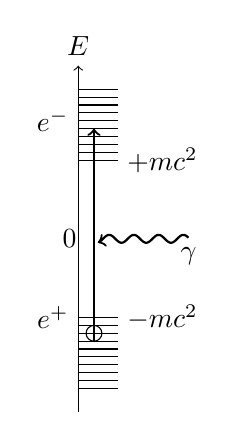
\begin{tikzpicture}[domain=-1.5:1.5]
  \draw[->] (0,-2.2) -- (0,2.2) node[above] {$E$};
  \foreach \x in {1.1, 1.2, 1.3, 1.4, 1.5, 1.6, 1.7, 1.8, 1.9}
    \draw[-] (0,\x) -- (0.5,\x) ;
  \foreach \x in {-1.1, -1.2, -1.3,-1.4, -1.5, -1.6, -1.7, -1.8, -1.9}
    \draw[-] (0,\x) -- (0.5,\x) ;
  \draw[-] (0,1) -- (0.5,1) node[right] {$+mc^2$};
  \draw[-] (0,-1) -- (0.5,-1) node[right] {$-mc^2$};
  \draw[-] (0.1,0) -- (0.1, 0) node[left] {$0$};
  \draw[domain= 0.25:1.4, samples=100, <-, thick] plot(\x, {0.05 * sin(20 * \x r) }) node [below] {$\gamma$};
  \draw[thick, ->] (0.2,-1.3) -- (0.2, 1.4);
  \draw (0.2, -1.2) circle (1mm); 
  \node [left] at (0, -1) {$e^+$};
  \node [left] at (0, 1.5) {$e^-$};
\end{tikzpicture}
\caption{Образование электрон-позитронной пары по действием $\gamma$-кванта. } \label{fig:14_2}
\end{figure}

Тогда переход электрона из состояния с отрицательной энергией $E_1 < 0$ в состояние с положительной энергией $E_2 > 0$ интерпретируется как \underline{рождение $e^-$, $e^+$-пары}: частицы (электрона) с энергией $E_2$ и античастицы (позитрона) с энергией $\abs{E_1}$. Обратный переход из состояния с положительной энергией $E_2 > 0$ в состояние с отрицательной энергией $E_1 < 0$, в котором выделяется энергия $\abs{E_1} + E_2$, интерпретируется как \underline{аннигиляция} (взаимное уничтожение) частицы и античастицы ($e^-$, $e^+$-аннигиляция с излучением $\gamma$-кванта). Вслед за предсказанием Дираком существования позитрона, Андерсон в 1932 г. обнаружил позитроны в космических лучах.

Таким образом, наличие четырех компонент волновой функции $\Psis$ означает, что каждое состояние может иметь два знака энергии (положительный и отрицательный) и два направления спина ($m_s = \pm \dfrac{1}{2}$, см. \S 3 главы \rom{8}). Столбец из четырех компонент для биспинора $\Psis(\vr, t)$ не связан с четырехмерностью пространства Минковского. 

\begin{sloppypar}
\section{Уравнение Дирака заряженной релятивистской частицы в электромагнитном поле. Уравнение Паули}
\end{sloppypar}

Обобщим уравнение Дирака на случай наличия внешнего электромагнитного поля, описываемого 4-потенциалом
$$
A^i=(\Phi, \vA)
$$

Функция Гамильтона заряженной частицы во внешнем электромагнитном поле в классической релятивистской механике имеет вид:
$$
H(\vr, \vec{P}, t) \equiv E = \sqrt{c^2\brc{\vec{P} - \frac{e}{c}\vA(\vr, t)}^2 + m^2c^4} + e\Phi(\vr, t),
$$
где обобщенный импульс $\vec{P}$ частицы связан с ее обычным импульсом $\vp$ формулой
$$
\vec{P} = \vec{p} + \frac{e}{c}\vA(\vr, t)
$$
(см.~\llref{16}{2})

Предполагая, что та же <<линеаризация корня>>, что и в пункте 1.1, справедлива и при наличии электромагнитного поля, применяя принцип соответствия между классическими величинами и операторами, получим  
\begin{equation}
\label{eq:14_3_1}
\boxed{i \hbar \pd{}{t} \Psis(\vr, t) = \brs{c(\aD, (\vec{P} - \frac{e}{c} \vA)) + \bD mc^2 + e\Phi} \Psis(\vr, t)}
\end{equation}

--- {\em уравнение Дирака для заряженной частицы во внешнем электромагнитном поле}. Здесь $\op{\vec{P}} = - i \hbar \nabla$, $\op{\vec{P}} - \frac{e}{c} \vA \equiv \plong$ --- оператор <<удлиненного>> импульса, заряд электрона $e < 0$.

Рассмотрим нерелятивистский предел уравнения Дирака \eqref{eq:14_3_1}. Считая состояние стационарным, запишем $\Psis(\vr, t) = e^{-\frac{iEt}{\hbar}} \psi(\vr)$, тогда
\begin{equation}
\label{eq:14_3_2}
\brs{E - c(\aD, \plong) - \bD mc^2 - e\Phi} \psi(\vr) = 0,
\end{equation}
где $\aD = \brc{\begin{matrix} \op{0}& \msigm \\ \msigm &  \op{0} \end{matrix}}$ , $\op{\beta} = \brc{\begin{matrix} \op{1}& \op{0} \\ \op{0} &  -\op{1} \end{matrix} }$.

Причем в дальнейшем будем считать $E>0$, т.~е. \underline{зафиксируем знак энергии} (в нерелятивистской квантовой механике имеются только состояния с положительной энергией). Представим далее волновую функцию в виде $\psi(\vr) = \brc{\begin{matrix} \phi(\vr) \\ \chi(\vr) \end{matrix}}$, где $\phi(\vr)$ и $\chi(\vr)$ --- двухкомпонентные функции (спиноры). Тогда уравнение \eqref{eq:14_3_2} разбивается на систему двух уравнений относительно спиноров $\phi(\vr)$ и $\chi(\vr)$:
\begin{gather}
\label{eq:14_3_3}
(E - mc^2 - e\Phi) \phi(\vr) = c(\msigm, \plong) \chi(\vr) \\
(E + mc^2 - e\Phi) \chi(\vr) = c(\msigm, \plong) \phi(\vr) \nonumber
\end{gather}
 
Исследуем систему \eqref{eq:14_3_3} в нерелятивистском пределе в слабых полях, т.~е $E \simeq mc^2 + \epsilon$, где $\epsilon$ --- {\em полная нерелятивистская энергия} и $\abs{\epsilon - e\Phi} \ll mc^2$, причем  
$$
\frac{\abs{\epsilon - e\Phi}}{mc^2} \sim \brc{\frac{v}{c}}^2 \ll 1
$$
В этом случае система \eqref{eq:14_3_3} перейдет в 
\begin{gather}
\label{eq:14_3_4}
(\epsilon - e\Phi) \phi(\vr) = c(\msigm, \plong) \chi(\vr) \\
\label{eq:14_3_5}
(2mc^2 + \epsilon - e\Phi) \chi(\vr) = c(\msigm, \plong) \phi(\vr)
\end{gather}

Из уравнения \eqref{eq:14_3_5} в низшем порядке нерелятивистского приближения находим:
\begin{equation}
\label{eq:14_3_6}
\boxed{\chi(\vr) \approx \frac{\cancel c (\msigm, \plong)}{2mc^{\cancel 2}} \phi(\vr)}
\end{equation}

Откуда видно, что в нерелятивистском приближении при $E > 0$:
%$$
%\underbrace{\frac{\abs{\chi(\vr)}}{\abs{\phi(\vr)}}}_{\text{<<большой>> или <<верхний>> спинор}} \sim %\frac{p}{mc}  \sim \frac{v}{c} \ll 1
%$$
$$
\frac{\abs{\chi(\vr)}}{\abs{\phi(\vr)}} \sim \frac{p}{mc}  \sim \frac{v}{c} \ll 1
$$
то есть спинор $\chi(\vr)$ имеет по отношению к $\phi(\vr)$ порядок малости $\dfrac{v}{c} \ll 1$. Это позволяет при $E > 0$ говорить о двух нижних компонентах дираковского спинора, т.~e. о $\chi(\vr)$, как о малых.
%При этом $\chi(\vr)$ - <<малый>> или <<нижний>> спинор.

Подставим далее приближенное выражение \eqref{eq:14_3_6} для $\chi(\vr)$ в уравнение \eqref{eq:14_3_4} системы и получим с линейной точностью по $\dfrac{v}{c}$ уравнение для двухкомпонентного спинора $\phi(\vr)$:
\begin{equation}
\label{eq:14_3_7}
(\epsilon - e\Phi)\phi(\vr) = \frac{1}{2m}(\msigm, \plong)(\msigm, \plong) \phi(\vr)
\end{equation}

\begin{excr}
Доказать, что
$$
(\msigm, \plong)(\msigm, \plong) = \plong^2 \op{1} - \frac{e\hbar}{c}(\msigm, \Hvec),
$$
где $\plong = \op{\vec{P}} - \dfrac{e}{c} \vA$, $\Hvec = rot \vA$.
\end{excr}

Преобразуем правую часть \eqref{eq:14_3_7}, используя это тождество. В результате получаем нерелятивистское уравнение, описывающее движение заряженной частицы по спином $1/2$ в электромагнитном поле:
\begin{equation}
\label{eq:14_3_8}
\boxed{\brs{\frac{1}{2m} (\op{\vec{P}} - \frac{e}{c} \vA)^2 - \frac{e\hbar}{2mc} (\msigm, \Hvec) + e\Phi}\phi(\vr) = \epsilon \phi(\vr)}
\end{equation}
--- {\em уравнение Паули} (1927 г.). Здесь $\phi(\vr)$ --- спинор Паули, т.~е. двухкомпонентная волновая функция. Две компоненты соответствуют двум возможным проекциям спина на произвольное направление. Сравнивая это уравнение с уравнением Дирака, отметим, что уравнение Дирака имеет 4 линейно независимых решения: $\xi = +1, \Lambda = \pm 1$ --- спиральность, т.~е. проекция спина частицы на направление её движения (2 спиновых состояния \underline{частицы}) и $\xi = -1, \Lambda = \pm 1$ (2 спиновых состояния \underline{античастицы}). В нерелятивистском приближении у энергии только один знак ($\xi = +1$ --- см. выше), поэтому здесь достаточно двухкомпонентной волновой функции.

Второе слагаемое в левой части \eqref{eq:14_3_8} отражает наличие спиновых свойств у электрона: это оператор взаимодействия собственного магнитного момента частицы с внешним полем $\Hvec$:
$$
- (\mmu, \Hvec) = - \frac{e\hbar}{2mc}(\msigm, \Hvec) = \mu_B (\msigm, \Hvec), 
$$
где $\mu_B = -\frac{e\hbar}{2mc}$ --- магнетон Бора ($e < 0$). Собственному магнитному моменту соответствует оператор
\begin{equation}
\label{eq:14_3_9}
\mmu = \frac{e\hbar}{2mc} \msigm = 2 \brc{\frac{e}{2mc}}\op{\vec{s}}
\end{equation}
%\mmu = \frac{e\hbar}{2mc} \msigm = 2 (\frac{e}{2mc})\underbrace{(\frac{\hbar\msigm}{2})}_{\op{\vec{s}}} = 2 \times \underbrace{(\frac{e}{2mc})}_{\text{гиромагнитное отношение}} \times \op{\vec{s}}

Выражение \eqref{eq:14_3_9} показывает, что для спинового (или собственного) момента в {\em гиромагнитном отношении} $g\brc{\dfrac{e}{2mc}}$ фактор $g = 2$, т.~е. гиромагнитное отношение (отношение магнитного момента частицы к угловому моменту) в 2 раза превышает аналогичную величину, связанную с орбитальным моментом.

Соответствующее предположение содержалось ещё в гипотезе Уленбека-Гаудсмита (1925 г.) и было использовано Паули при написании его (феноменологического!) уравнения \eqref{eq:14_3_8}, но оказалось, что этот результат есть простое следствие теории Дирака. В этом состоит огромное достоинство теории Дирака: уравнение Дирака уже содержит спиновые (магнитные) свойства электрона, а уравнение Паули представляет собой лишь нерелятивистский предел уравнения Дирака!

Математически переход к нерелятивистскому приближению уравнения Дирака означает пренебрежение <<нижними>> (<<малыми>> $O(v/c)$) компонентами дираковской волновой функции и переход к подпространству только <<больших>> (или <<верних>>) компонент.

\section{Релятивистские поправки к уравнению Шрёдингера частицы во внешнем электромагнитном поле. Спин-орбитальное взаимодействие}

В предыдущем параграфе мы преобразовали уравнение Дирака, предполагая, что оно описывает нерелятивистскую частицу. При этом мы удерживаем слагаемые первого порядка по малому параметру $v/c \ll 1$. В результате было получено уравнение Паули. Рассмотрим теперь нерелятивистский предел уравнения Дирака для заряженной частицы, движущейся в электромагнитном поле. Например, если электрон движется в поле неподвижного протона в атоме H, то $e\Phi = U(\vr) = -\dfrac{e^2}{r}$, $\vA = 0$ и $\Hvec = 0$. В отсутствие магнитного поля уравнение Паули \eqref{eq:14_3_8} переходит в обычное нерелятивистское уравнение Шрёдингера.
$$
\brs{\frac{\op{\vp}^2}{2m} + U(\vr)}\phi(\vr)=\epsilon \phi(\vr)
$$
для частицы в потенциальном поле $U(\vr)$. Таким образом, согласно теории Дирака не существует поправок первого порядка по $v/c \ll 1$ к энергиям стационарных состояний атома водорода (и любой другой системы, где частица движется в электромагнитном поле).

Предположим, что такие поправки существуют во втором порядке по малому параметру $v/c$. Заметим, что для электрона в атоме водорода
$$
\frac{v_{\text{ат}}}{c} \sim \frac{p}{mc} \sim \frac{\hbar}{m c a_B} = \left | a_B = \frac{\hbar^2}{m e^2}\right | = \frac{e^2}{\hbar c} = \alpha \simeq \frac{1}{137}
$$
--- {\em постоянная тонкой структуры атомных спектров} т.~е. $v_{\text{ат}} \ll c$ и для описания атомных процессов нет необходимости привлекать точный гамильтониан Дирака. Достаточно найти приближённый вид уравнения по степеням разложения $v/c$ вплоть до $\brc{v/c}^2$, т.~е. до $\alpha^2$.

Вернёмся к уравнению \eqref{eq:14_3_5}, из которого следует
\begin{equation}
\label{eq:14_4_1}
\chi(\vr) = \frac{c(\msigm \op{\vp})}{2mc^2 + \epsilon - e\Phi} \phi(\vr) 
\end{equation}

Далее рассмотрим следующее за \eqref{eq:14_3_6} нерелятивистское приближение
$$
(2mc^2 + \epsilon - e\Phi)^{-1} = \brcr{2mc^2 \brc{1 + \brc{\frac{\epsilon - e\Phi}{2mc^2}}}}^{-1} \approx \frac{1}{2mc^2} \brc{1 - \frac{\epsilon - e\Phi}{2mc^2}},
$$
где, как отмечалось выше, $\dfrac{\abs{\epsilon - e\Phi}}{mc^2} \sim \dfrac{v^2}{c^2} \ll 1$.

Тогда из \eqref{eq:14_3_4} и \eqref{eq:14_4_1} получаем:
$$
\brc{\epsilon - e\Phi}\phi(\vr) = c (\msigm, \op{\vp}) \chi(\vr) = \brcr{\frac{\cancel{c^2} (\msigm, \op{\vp})}{2m \cancel{c^2}}\brc{1 - \frac{\epsilon - e\Phi}{2mc^2}}(\msigm, \op{\vp})} \phi(\vr)
$$

Так как $(\msigm, \vp)^2 = \op{\vp}^2$, то
\begin{equation}
\label{eq:14_4_2}
\brs{\epsilon - U(r) - \frac{\op{\vp}^2}{2m}}\phi(\vr) = \underbrace{-\brs{(\msigm, \op{\vp})\brc{\frac{\epsilon - U(\vr)}{4m^2c^2}}(\msigm, \op{\vp})}}_{\op{V}_{\text{кв. рел.}} \sim (v/c)^2} \phi(\vr)
\end{equation}

Левая часть уравнения \eqref{eq:14_4_2} напоминает нерелятивистское уравнение Шрёдингера. Однако для того, чтобы перейти от \eqref{eq:14_4_2} к уравнению Шрёдингера, необходимо учесть, что с точностью до членов порядка $\brc{v/c}^2$ спинор $\phi(\vr)$ уже не может служить нерелятивистской волновой функцией, т.~к. он неправильно нормирован. Действительно, если биспинор $\Psis = \brc{\begin{matrix} \phi \\ \chi \end{matrix}}$ уже был нормирован на единицу, то
$$
1 = \int \diff\vr \Psis^\dag \Psis = \int \diff\vr (\phi^\dag \phi + \chi^\dag \chi),
$$
где $\phi^\dag = (\phi_1^*,~~~\phi_2^*)$.

Поскольку сюда входит $\chi^\dag \chi$, <<малый>> спинор $\chi$ достаточно взять в первом по $v/c$ порядке, т.~е. в форме \eqref{eq:14_3_6}:
$$
\chi(\vr) \simeq \frac{(\msigm \op{\vp})}{2mc}\phi(\vr)
$$

Условие нормировки принимает вид
\begin{gather*}
\int \diff\vr \brc{\phi^\dag \phi + \phi^\dag \frac{(\msigm \op{\vp})^\dag}{2mc} \frac{(\msigm \op{\vp})}{2mc} \phi} = 1
\end{gather*}
или с учетом эрмитовости оператора $\msigm \op{\vp}$ и $(\msigm \op{\vp})^2 = \op{\vp}^2$
$$
\int \diff\vr \phi^\dag \left(\op{1} + \frac{\op{\vp}^2}{4m^2c^2}\right) \phi = 1  
$$

Как видим, в рассматриваемом приближении
$$
\bk{\phi}{\phi} \neq 1
$$

В то же время
$$
\bfkh{\phi}{\op{1} + \frac{\op{\vp}^2}{4m^2c^2}}{\phi} = 1,
$$
т.~е. с точностью до слагаемых второго порядка по $v/c$ имеем:
$$
\bfkh{\phi}{\brc{\op{1} + \frac{\op{\vp}^2}{8m^2c^2}}^2}{\phi} = 1
$$
или
$$
\bkh{\brc{\op{1} + \frac{\op{\vp}^2}{8m^2c^2}}\phi}{\brc{\op{1} + \frac{\op{\vp}^2}{8m^2c^2}}\phi} = 1
$$

Таким образом, естественно ввести двухкомпонентную волновую функцию (спинор Паули):
$$
\psi_\Pi = \brc{\op{1} + \frac{\op{\vp}^2}{8m^2c^2}} \phi,
$$
нормированную на единицу
$$
\bk{\psi_\Pi}{\psi_\Pi} = 1
$$

С точностью до слагаемых второго порядка малости по $v/c$ спинор $\phi$ выражается через спинор Паули следующим образом:
\begin{equation}
\label{eq:14_4_3}
\phi = \brc{\op{1} + \frac{\op{\vp}^2}{8m^2c^2}}^{-1} \psi_\Pi \simeq \brc{\op{1} - \frac{\op{\vp}^2}{8m^2c^2}} \psi_\Pi
\end{equation}

Выведем уравнение, определяющее спинор Паули $\psi_\Pi$. Для преобразования правой части \eqref{eq:14_4_2} воспользуемся результатом следующего упражнения:

\begin{excr}
Используя соотношение 
$$
[\msigm \op{\vp}, f(r) \msigm \op{\vp}] = -i\hbar (\msigm, \nabla f)(\msigm, \op{\vp}),
$$
показать, что
$$
(\msigm, \op{\vp}) U(r) (\msigm, \op{\vp}) = U(r) \op{\vp}^2 - i \hbar (\nabla U(r), \op{\vp}) + \hbar \msigm [\nabla U(r) \times \op{\vp}]
$$
\end{excr}

Уравнение \eqref{eq:14_4_2} принимает вид
$$
\brs{\epsilon - U(r) - \frac{\op{\vp}^2}{2m}}\phi(\vr) =
$$
$$
\brs{- \frac{\epsilon - U(r)}{4m^2c^2}\op{\vp}^2 + \frac{1}{4m^2 c^2} \brc{-i\hbar (\nabla U(r) \op{\vp}) + \hbar \msigm [(\nabla U) \times \op{\vp}]}} \phi(\vr)
$$
или с учётом \eqref{eq:14_4_3} имеем:
$$
\brs{\epsilon - U(r) - \frac{\op{\vp}^2}{2m}}\brc{\op{1} - \frac{\op{\vp}^2}{8m^2c^2}} \psi_\Pi = \brs{- \frac{\epsilon - U(r)}{4m^2c^2}\op{\vp}^2 + \frac{1}{4m^2 c^2} \brc{\dots}}
$$

Собирая в правой части слагаемые $\sim (v/c)^2$, получим:
$$
\brs{\epsilon - U(r) - \frac{\op{\vp}^2}{2m}}\psi_\Pi = \brs{- \frac{\epsilon - U(r)}{8m^2c^2}\op{\vp}^2 -\frac{\op{\vp}^4}{16m^3 c^2}+ \frac{1}{4m^2 c^2} \brc{\dots}} \psi_\Pi,
$$
где 
\begin{equation}
\label{eq:14_4_4}
\brc{\dots} = -i\hbar (\nabla U(r), \op{\vp}) + \hbar \msigm [(\nabla U) \times \op{\vp}]
\end{equation}

В центрально-симметричном поле $\nabla U(r) = \dfrac{dU}{dr} \dfrac{\vr}{r}$, поэтому 
$$
\hbar \msigm [(\nabla U) \times \op{\vp}] = \hbar \frac{1}{r} \D{U}{r} \msigm [\vr \times \vp] 
$$

$\vec{L} = \hbar \vec{l}$ --- оператор орбитального момента частицы (см. \S 4 главы \rom{8})

Продолжим равенство выше:
$$
\hbar \frac{1}{r} \D{U}{r} \msigm [\vr \times \vp] = {\hbar} \frac{1}{r} \D{U}{r} (\msigm, \op{\vec{L}}) = \frac{2}{r} \D{U}{r} (\op{\vec{S}}, \op{\vec{L}})
$$

Поэтому в правой части \eqref{eq:14_4_4} оператор 
$$
\frac{\hbar \msigm}{4m^2c^2} [(\nabla U) \times \op{\vp}] = \frac{\hbar}{2m^2c^2}\frac{1}{r} \D{U}{r} (\op{\vec{s}} \cdot \op{\vec{l}}) = \op{V}_{SO}
$$
называют оператором спин-орбитального взаимодействия. Для движения электрона в кулоновском поле ядра с зарядом $-Ze$:
$$
U(r) = -\frac{Ze^2}{r},
$$
получаем выражение, определяющее характерную величину спин-орбитального взаимодействия в атоме:
\begin{gather*}
\boxed{A_{SO} (r) = \frac{Ze^2 \hbar^2}{2m^2 c^2 r^3} > 0}
\end{gather*}

Происхождение спин-орбитального взаимодействия можно пояснить следующими полуклассическими рассуждениями. Пусть частица с зарядом $e$ и собственным магнитным моментом $\mmu = \frac{e}{mc}\hbar \op{\vec{s}}$ (см. \eqref{eq:14_3_9}) движется в центрально-симметричном электростатическом поле, которое определяется потенциалом $\Phi(r)$, т.~е. потенциальная энергия частицы есть $U(r)=e\Phi(r)$. Предположим, что в точке $\vr$ частица имеет скорость $\vec{v}$ и, соответственно, орбитальный момент $\vec{L} = m[\vr \times \vec{v}]$ (см. \autoref{fig:14_3}).

\begin{figure}[h!]
\centering
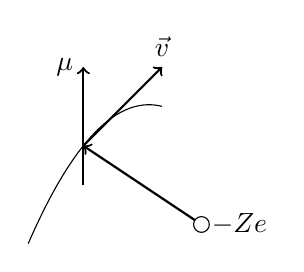
\begin{tikzpicture}[domain=-2:2]
  \draw[->, thick] (0, 0) -- (1, 1) node[above] {$\vec{v}$};
  \draw[->, thick] (0, -0.5) -- (0,1) node[left] {$\bm{\mu}$};
  \draw[<-, thick, shorten >= 3] (0, 0) -- (1.5,-1) node[right] {$-Ze$};
  \node at (1.3, -0.4) {$\vr$};
  \draw[domain=-0.7:1, samples=50] plot(\x,{-0.75 * \x * \x + 1.25 * \x});
  \draw (1.5, -1) circle (1mm); 
\end{tikzpicture}
\caption{К вопросу о спин-орбитальном взаимодействии.} \label{fig:14_3}
\end{figure}

Напряжённость электрического поля в этой же точке равна
$$
\vec{E} = - \nabla \Phi(r) = -\D{\Phi}{r} \frac{\vr}{r}
$$

В системе покоя частицы имеется магнитное поле, напряжённость которого с точностью до первого порядка по $v/c$ определяется формулой из курса <<Теория поля>> (\llref{24}{2}).

$$
\Hvec' = \frac{1}{c}[\vec{E} \times \vec{v}]
$$

Таким образом, возникает энергия взаимодействия магнитного момента с магнитным полем
$$
\op{V_m} = - \mu \Hvec' = \brc{-\frac{e\hbar}{mc}} \frac{1}{r}\brc{-\frac{1}{c} \D{\Phi}{r}}\brc{\op{\vec{s}} [\vr \times \vec{v}]} = {\frac{\hbar^2}{m^2c^2} \frac{1}{r} \D{U(r)}{r} (\vec{s} \cdot \vec{l})},
$$
которая с точностью до численного коэффициента согласуется с видом оператора $\op{V}_{SO}$.

Приведём уравнение \eqref{eq:14_4_4} к окончательному виду, воспользовавшись результатом упражнения.
\begin{excr}
Доказать, что в пределах требуемой точности $\brc{\dfrac{v}{c}}^2$: 
$$
(\epsilon - U(r)) \op{\vp}^2 = \frac{\op{\vp}^4}{2m} - \hbar^2 \Delta U(r) - 2i\hbar(\nabla U(r), \op{\vp})
$$
\end{excr}

Тогда
\begin{gather*}
\brs{\epsilon - U(r) - \frac{{\vp}^2}{2m}}\psi_\Pi = \brs{ -\frac{\op{\vp}^4}{8m^3c^2} + \frac{1}{8} \brc{\frac{\hbar}{mc}}^2 \Delta U(r) + \op{V}_{SO}} \psi_\Pi
\end{gather*}
или
$$
\brs{\epsilon - U(r) - \frac{{\vp}^2}{2m}}\psi_\Pi = \op{V}_{\text{кв. рел.}} \psi_\Pi,
$$
где 
\begin{equation}
\label{eq:14_4_5}
\op{V}_{\text{кв. рел.}} = \op{V}_1 + \op{V}_2 + \op{V}_{SO}
\end{equation}

Приближение, учитывающее поправки к гамильтониану $\op{H}_\Pi$ второго порядка по $\dfrac{v}{c} \ll 1$, носит название \underline{квазирелятивистского}. Влияние операторов $\op{V}_1$, $\op{V}_2$ и $\op{V}_{SO}$ на энергии стационарных состояний может быть исследовано в рамках теории возмущений.

Оператор
$$
V_1 = -\frac{\op{\vp}^4}{8m^3c^2}
$$ 
может быть интерпретирован как \underline{релятивистская поправка к оператору кинетической энергии}. В самом деле, кинетическая энергия $K$ --- это разность полной энергии $E$  и энергии покоя $mc^2$. В нерелятивистском случае имеем:
$$
K = \sqrt{m^2c^4 + c^2p^2} - mc^2 = mc^2\brc{1 + \frac{\op{\vp}^2}{m^2c^2}}^{1/2} - mc^2 \approx
$$
$$
\approx mc^2\brc{1 + \frac{\op{\vp}^2}{2m^2c^2} - \frac{\op{\vp}^4}{8m^2c^4}} - mc^2 = \frac{\op{\vp}^2}{2m} - \frac{\op{\vp}^4}{8m^3c^2},
$$
т.~е. оператор $\op{V_1}$ отражает релятивистскую зависимость кинетической энергии электрона от импульса.

Оператор $\op{V_2} = \dfrac{1}{8} \brc{\dfrac{\hbar}{mc}}^2\Delta U(r)$ (оператор Дарвина, 1928 г.) отражает контактное взаимодействие электрона с ядром. Действительно, в случае движения электрона в атоме в кулоновском поле ядра $U(r)  = -\dfrac{Ze^2}{r}$ имеем:
$$
\Delta U(r) = -Ze^2 \Delta \brc{\frac{1}{r}} = 4 \pi Ze^2 \delta(\vr)
$$

Тогда оператор $\op{V_2}$ принимает вид
$$
\op{V_2} = \frac{\pi}{2} \brc{\frac{\hbar}{mc}}^2 Ze^2 \delta(\vr),
$$
из которого следует, что $\avg{\op{V_2}} \neq 0$ только при непосредственной близости электрона к ядру или <<в контакте с ядром>>, когда $\vr = 0$. Оператор $\op{V_2}$ приведёт к сдвигу энергии тех состояний, для которых $\avg{\op{V_2}} \sim \abs{\psi(0)}^2 \neq 0$, т.~е. для $s$-состояний ($l=0$). Напротив, спин-орбитальное взаимодействие $\avg{\op{V}_{SO}} \sim \avg{(\op{\vec{s}} \cdot \op{\vec{l}})}$ отлично от нуля для состояний с $l \neq 0$.
